These problems are here to jar you and make you acknowldge the complexity of even that which is simple:

\tikzstyle{vertex}=[circle,draw,minimum size=0.5cm]
\begin{exercises}
    \begin{questions}
        \Question[2] Place the numbers 1,2,3, 4 and 5 in the circles of the following figure so that no two adjacent numbers (that is, numbers with a difference that is 1 ) are connected by a line.
        \begin{center}
        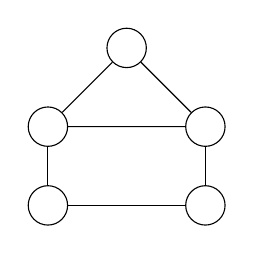
\begin{tikzpicture}
            \node (d) at (0,0) [vertex] {};
            \node (e) at (2,0) [vertex]  {};
            \node (b) at (0,1) [vertex]  {};
            \node (c) at (2,1) [vertex]  {};
            \node (a) at (1,2) [vertex]  {};
            \draw (a) -- (b) -- (c);
            \draw (c) -- (e);
            \draw (d) -- (e);
            \draw (b) -- (d);
            \draw (a) -- (c);
        \end{tikzpicture}
        \end{center}
        \Question[2] A palindromic number is a whole number that is unchanged when the order of the digits is reversed, for example, 131 and 34 543. The number 39793 is palindromic. Find the next 5 palindromic numbers.
        \begin{solutionordottedlines}[1in]
        \end{solutionordottedlines}
        \Question[2] Complete the following magic square, in which each row, column and diagonal must add up to the same sum.
            \begin{center}
                \begin{tabular}{|l|l|l|}
                    \hline
                    19 &  &  \\
                    \hline
                     & 15 &  \\
                    \hline
                    22 &  & 11 \\
                    \hline
                \end{tabular}
            \end{center}
        \Question[2] Place the numbers 1 to 9 in each of the circles in the following figure so that the sums of the numbers on each straight line are equal.
        \begin{center}
        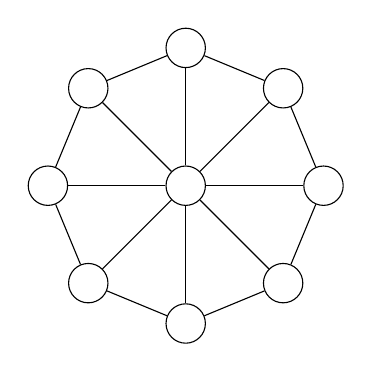
\begin{tikzpicture}[scale=0.7]
          \def\radius{2.5cm}
          \node (o) at (0,0) [vertex] {};
          
          \foreach \a in {1,2,...,8}{
            \node (n\a) at (\a*360/8: \radius) [vertex] {};
            \draw (n\a) -- (o);
          }
          
          \foreach \b [remember=\b as \lastb (initially 8)] in {1,2,...,8}{
            \draw (n\b) -- (n\lastb);
          }
        \end{tikzpicture}
        \end{center}
        \Question[3] To protect his money from pickpockets, a merchant keeps his coins in several pouches so that he can pay any amount without revealing how much money he has, just by handing over the correct pouches. On the first day of trading he has six coins, so he places one coin in the first pouch, two coins in the second, and three coins in the third. This allows him to pay any value from one to six coins without having to open a pouch. The next day of trading he has 23 coins and five pouches. How should he distribute the coins to ensure that he can pay any amount from 1 to 23 coins?
            \begin{solutionordottedlines}[2in]
            \end{solutionordottedlines}
        \Question[3] It is possible to choose four numbers such that any value between 1 and 40 can be made by taking one or more of these numbers and adding or subtracting them from each other. Find the four numbers, and show how the values from 1 to 40 can be made.
        \question Using all the digits \(0,1,2,3,4,5,6,7,8\) and 9 , form two 5 -digit numbers so that their sum is:
        \begin{parts}
            \Part[1] the greatest possible
            \Part[1] the smallest possible
        \end{parts}
        \Question[3] Find the sum of whole numbers from 1 to 100.
        \begin{solutionorbox}[2in]
        \end{solutionorbox}
    \end{questions}
\end{exercises}

